%% LaTeX Beamer presentation template (requires beamer package)
%% see http://latex-beamer.sourceforge.net/
%% idea contributed by H. Turgut Uyar
%% template based on a template by Till Tantau
%% this template is still evolving - it might differ in future releases!

\documentclass[14pt]{beamer}

\mode<presentation>
%\mode<handout>
{
\usetheme{Berlin}

\setbeamercovered{transparent}
}

\usepackage[ngerman]{babel}
\usepackage[utf8]{inputenc}
\usepackage{tikz}					        % tikz-grafiken
\usetikzlibrary{shapes.multipart,trees,arrows,shapes,fit,backgrounds,topaths,positioning,fadings,decorations,automata}
\usepackage{pgfbaselayers}                  % GFX-Layer


% font definitions, try \usepackage{ae} instead of the following
% three lines if you don't like this look
%%%\usepackage{mathptmx}
%%%\usepackage[scaled=.90]{helvet}
%%%\usepackage{courier}

\ifx\pdftexversion\undefined
\usepackage[dvips]{graphicx}
\else
\usepackage{graphicx}
\DeclareGraphicsRule{*}{mps}{*}{}
\fi

\usepackage{listings}
\usepackage{xcolor}

\usepackage{wrapfig}
\usepackage{textcomp}
\usepackage{graphics}
%\usepackage{makeidx}
%\usepackage{mathpazo}
%\usepackage{multicol}
%\usepackage{srcltx}
\usepackage{color}

% via <http://anthony.liekens.net/index.php/LaTeX/SubscriptAndSuperscriptInTextMode>
\newcommand{\superscript}[1]{\ensuremath{^{\textrm{#1}}}}
\newcommand{\subscript}[1]{\ensuremath{_{\textrm{#1}}}}

\usepackage{eurosym}


\title{Split-Access-Routing und Priorisierung auf Linux-Basis}

%\subtitle{}

% - Use the \inst{?} command only if the authors have different
%   affiliation.
%\author{F.~Author\inst{1} \and S.~Another\inst{2}}
\author{Oluf~Lorenzen\inst{}}

% - Use the \inst command only if there are several affiliations.
% - Keep it simple, no one is interested in your street address.
\institute
{
axxeo GmbH
}

\date{Januar 2010}


% This is only inserted into the PDF information catalog. Can be left
% out.
%%%\subject{Talks}



% If you have a file called "university-logo-filename.xxx", where xxx
% is a graphic format that can be processed by latex or pdflatex,
% resp., then you can add a logo as follows:

\pgfdeclareimage[height=0.8cm]{axxeo_logo}{axxeo_logo}
 \logo{\pgfuseimage{axxeo_logo}}



% Delete this, if you do not want the table of contents to pop up at
% the beginning of each subsection:
%%\AtBeginSubsection[]
%{
%\begin{frame}<beamer>
%\frametitle{Vorgehensweise}
%\tableofcontents[currentsection,currentsubsection]
%\end{frame}
%}

% If you wish to uncover everything in a step-wise fashion, uncomment
% the following command:

%\beamerdefaultoverlayspecification{<+->}

\begin{document}

\begin{frame}
\titlepage
\end{frame}

\begin{frame}
\frametitle{Gliederung}
\tableofcontents
% You might wish to add the option [pausesections]
\end{frame}

\section{Installationsumfeld}

\begin{frame}
\frametitle<presentation>{Installationsumfeld}
%\begin{center}Messungen an Lebewesen und den dazu erforderlichen Mess- und Auswerteverfahren\end{center}
\begin{itemize}
 \item 4 Mitarbeiter
\item Linux-Server für Geschäftskunden
\begin{itemize}
 \item als Gateway ins Internet
\item Spam- und Viren-Scan
\item Routing und VPN
\end{itemize}
\item Support/Wartung über SSH (Secure Shell)
\end{itemize}

\end{frame}

\section{Ist-Zustand}
\subsection*{}
\begin{frame}
\frametitle{Ist-Zustand}
\begin{columns}[c]
  \column{1.8in}

\begin{footnotesize}  \begin{itemize}
    \item 2Mbit SDSL
    \item 4 Arbeitsplätze, 2 Server
    \item Wartung via SSH
    \item geringer HTTP-Traffic
  \end{itemize}\end{footnotesize}

  \column{1.8in}
\begin{figure}[h!]
      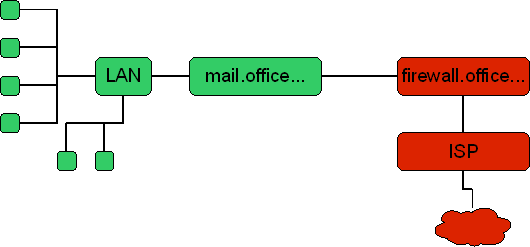
\includegraphics[width=1\textwidth]{GFX/netzplan}
  \end{figure}
\end{columns}
\end{frame}

\begin{frame}
\begin{columns}[c]
  \column{1.8in}

\begin{footnotesize}  \begin{itemize}
    \item 2Mbit SDSL
    \item 5-7 Arbeitsplätze, 2 Server
    \item Wartung via SSH
    \item viel (HTTP-)Traffic
  \end{itemize}\end{footnotesize}

  \column{1.8in}
\begin{figure}[h!]
      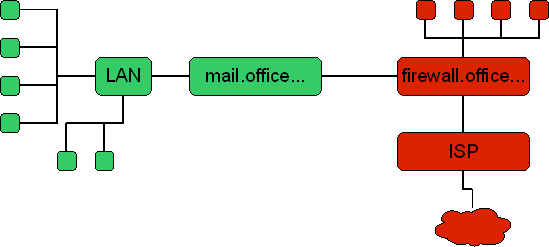
\includegraphics[width=1\textwidth]{GFX/netzplan_neu}
  \end{figure}
\end{columns}
\end{frame}

\section{Soll-Zustand}
\subsection*{}
\begin{frame}
\frametitle{Soll-Zustand}
\begin{itemize}
 \item auf Debian basierte Lösung
\item LARTC (Linux Advanced Routing \& Traffic Control)
\item \texttt{tc}\\
\item Arbeit bei Netzwerkauslastung möglich
\item Nutzung einer zweiten Anbindung
\end{itemize}
\end{frame}

\begin{frame}
\begin{figure}[h!]
      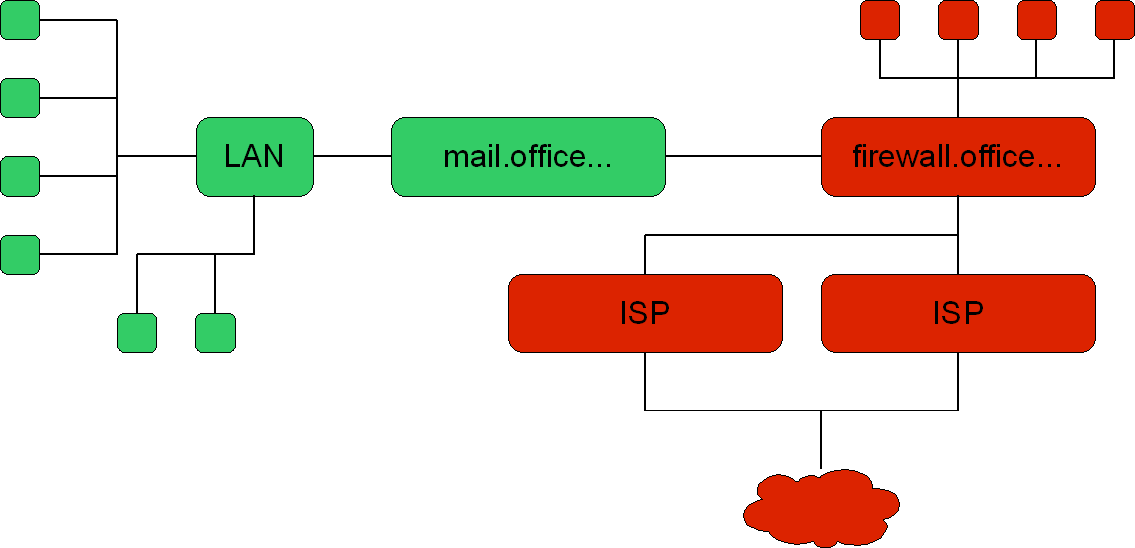
\includegraphics[width=1\textwidth]{GFX/netzplan_soll}
  \end{figure}
\end{frame}



\section{Durchführung}
\subsection{Split-Access-Routing}
\begin{frame}
\frametitle<presentation>{Split-Access-Routing}
 \begin{itemize}
    \item LARTC
    \item 2 Routing-Tabellen
    \item eine Default-Route für jede Tabelle
    \item modifizierte \emph{normale} Default-Route
    \item Aufteilung des Verkehrs von eins zu eins
  \end{itemize}
\end{frame}


\subsection{Priorisierung}
\begin{frame}%[plain]
\frametitle<presentation>{Priorisierung}
\texttt{tc}-Befehle:

\begin{tiny}
\end{tiny}
\lstset{basicstyle=\tiny, showstringspaces=false, tabsize=2,breaklines=true}
  \lstinputlisting[label=lst:tc]{Quellcode/tc.txt}

$\Rightarrow$ schwer verständlich, unleserlich \dots
\end{frame}


\begin{frame}%[plain]
\texttt{tcng}-Script:

\lstset{language=C, basicstyle=\tiny, showstringspaces=false, tabsize=2,breaklines=true}
  \lstinputlisting[label=lst:eth1_tcc]{Quellcode/eth1.tcc}

$\Rightarrow$ C-ähnliche Syntax (Syntaxhighlighting!), lesbar, schnell erweiterbar \dots
\end{frame}


\subsection{HTB}
\subsubsection{Selektierung}
\begin{frame}
\frametitle<presentation>{Traffic-Kategorisierung}
\begin{figure}[h!]
      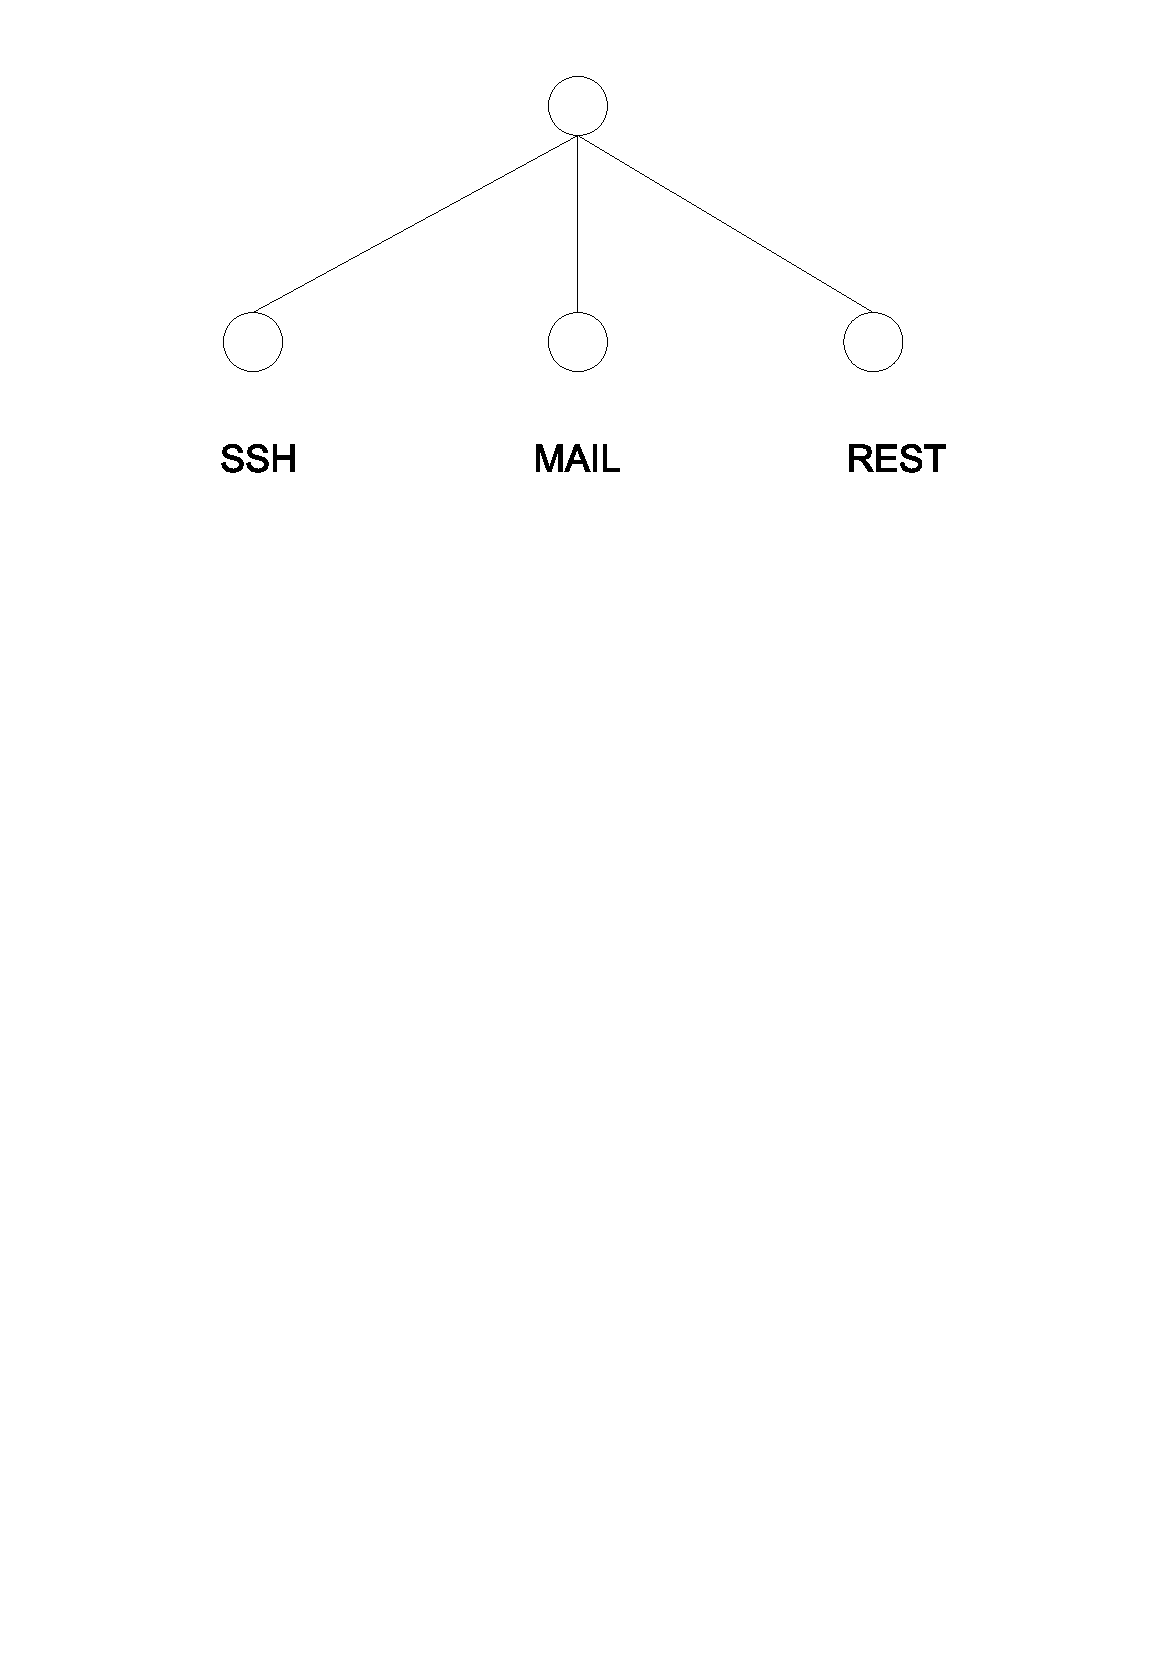
\includegraphics[width=1\textwidth]{GFX/bucket-hiracy-ssh-http-rest}
  \end{figure}
\end{frame}

\begin{frame}
\begin{figure}[h!]
      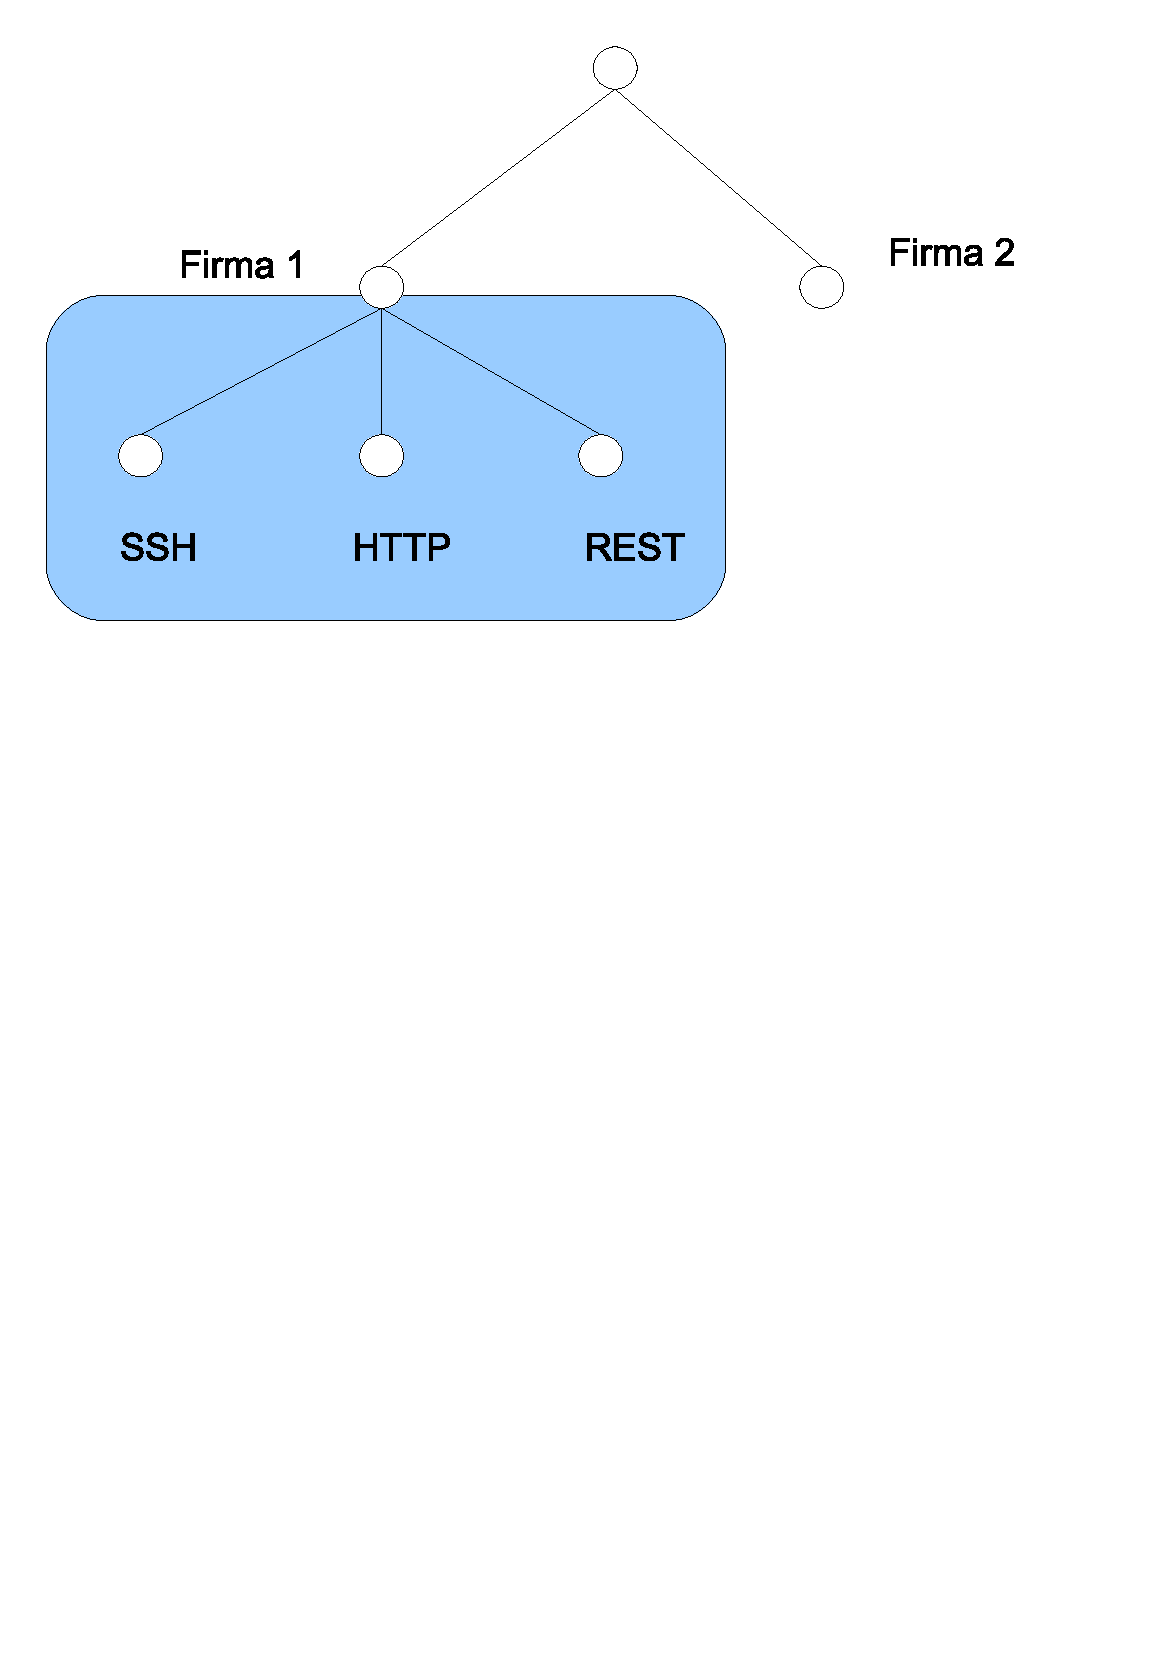
\includegraphics[width=1\textwidth]{GFX/bucket-hiracy-firma1-firma2}
  \end{figure}
\end{frame}

\begin{frame}
\begin{figure}[h!]
      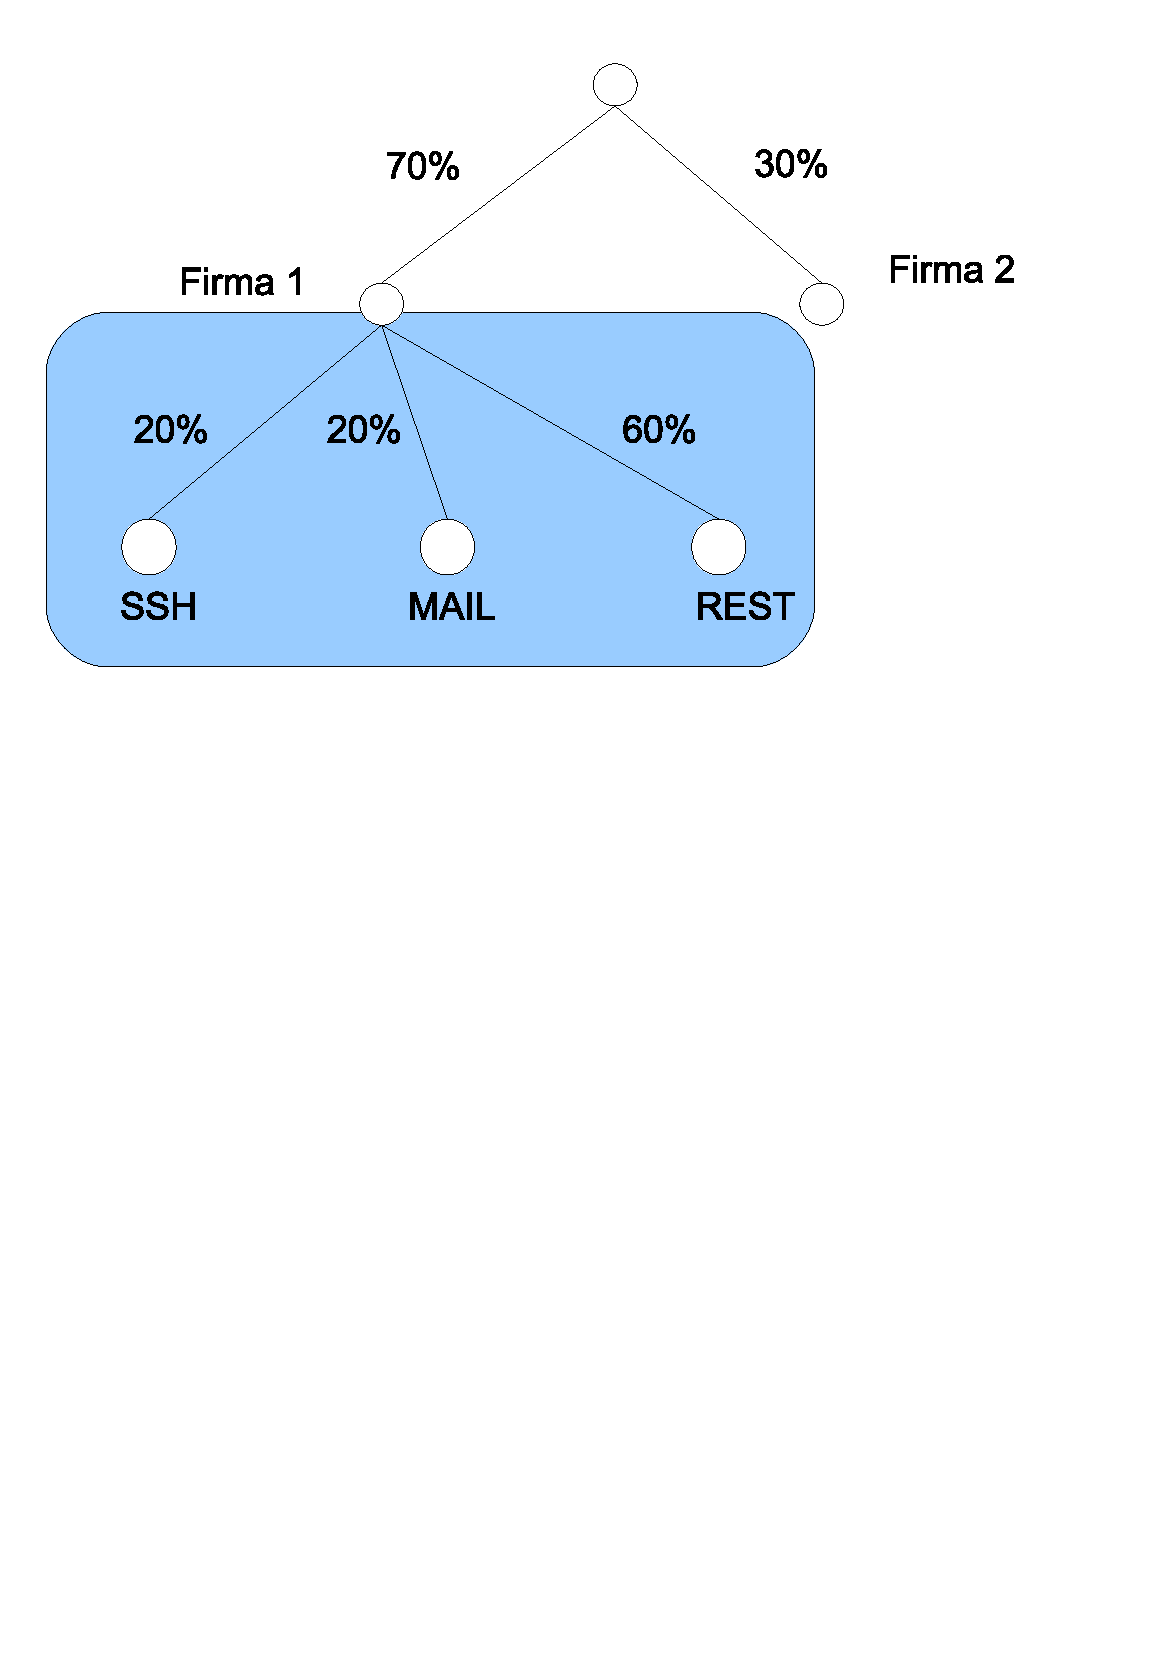
\includegraphics[width=1\textwidth]{GFX/bucket-hiracy-menge}
  \end{figure}
\end{frame}


\begin{frame}
\begin{figure}[h!]
      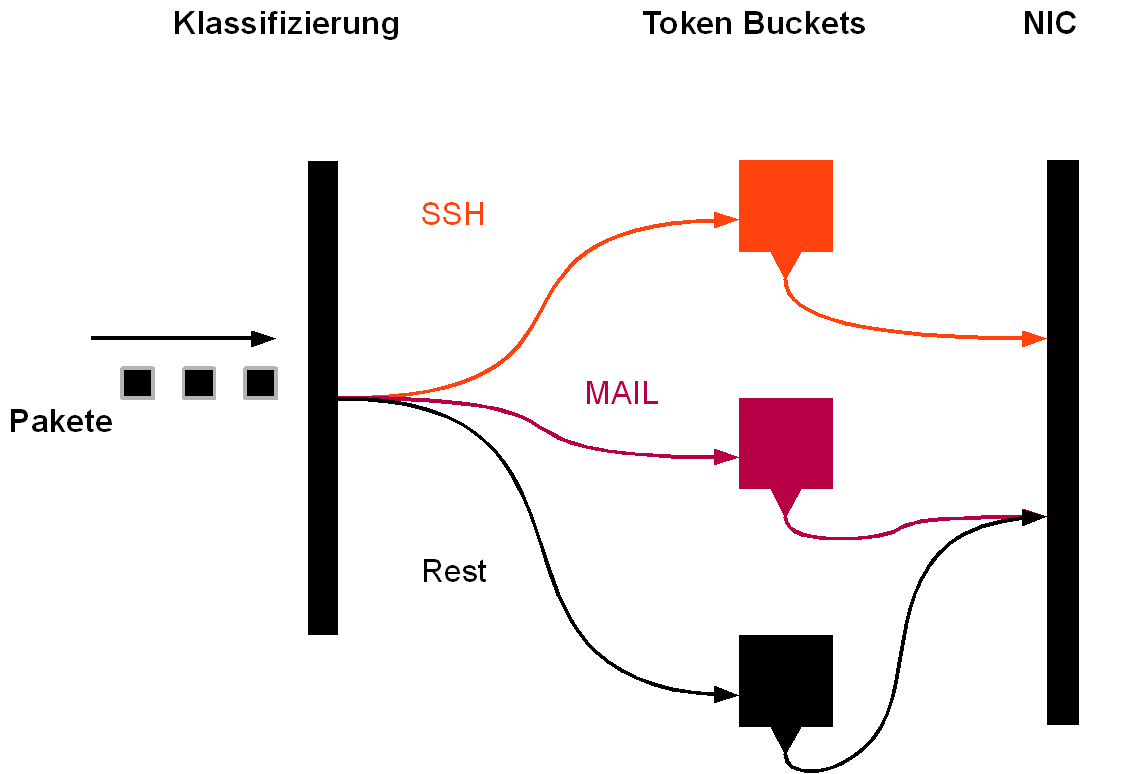
\includegraphics[width=1\textwidth]{GFX/htb-classification}
  \end{figure}
\end{frame}


\subsubsection{Token-Bucket}
\begin{frame}
\frametitle{Token-Bucket}
\begin{figure}[h!]
      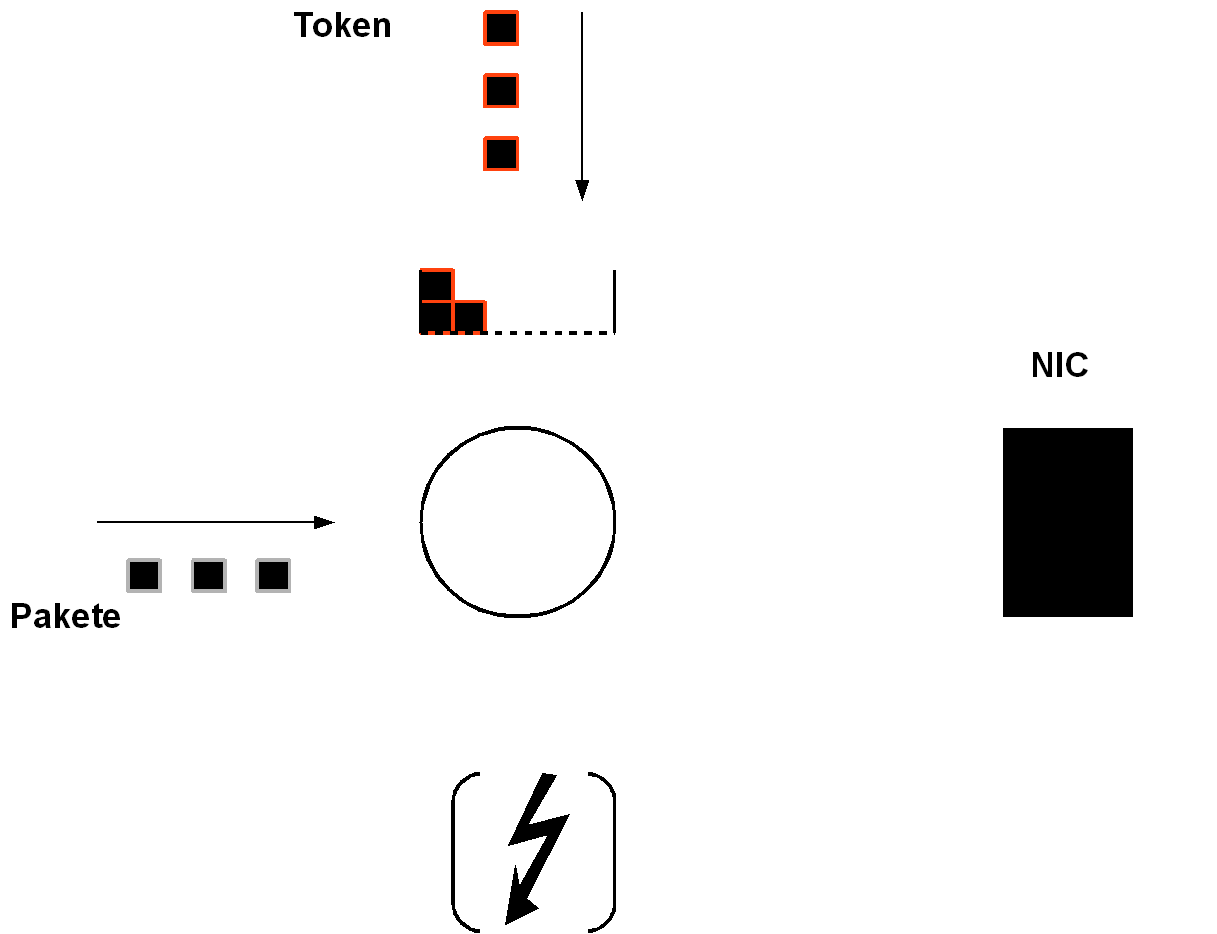
\includegraphics[width=0.7\textwidth]{GFX/tb-beginning}
  \end{figure}
\end{frame}


\begin{frame}
\begin{figure}[h!]
      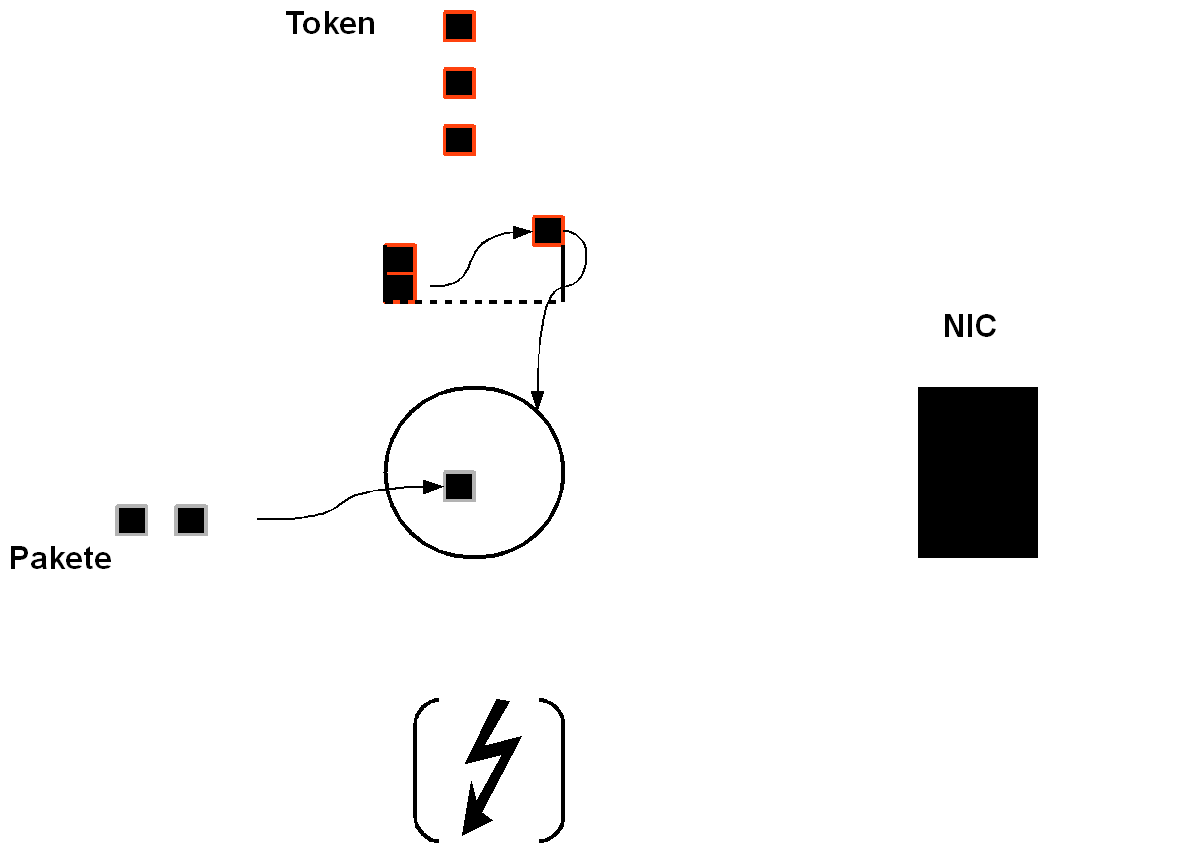
\includegraphics[width=0.7\textwidth]{GFX/tb-token-taken}
  \end{figure}
\end{frame}

\begin{frame}
\begin{figure}[h!]
      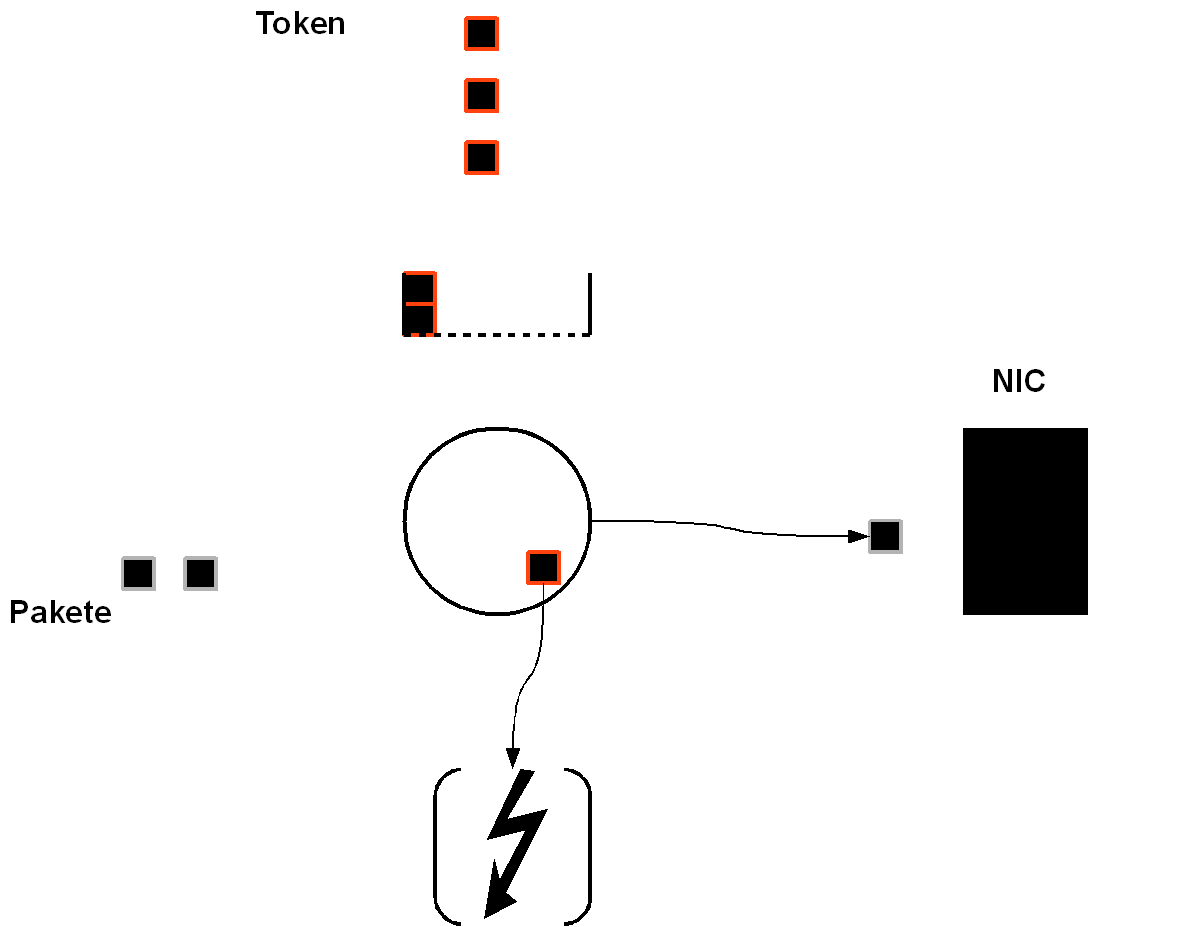
\includegraphics[width=0.7\textwidth]{GFX/tb-token-finished}
  \end{figure}
\end{frame}


\begin{frame}
\frametitle{Token Buckets \& Selektierung}
\begin{figure}[h!]
      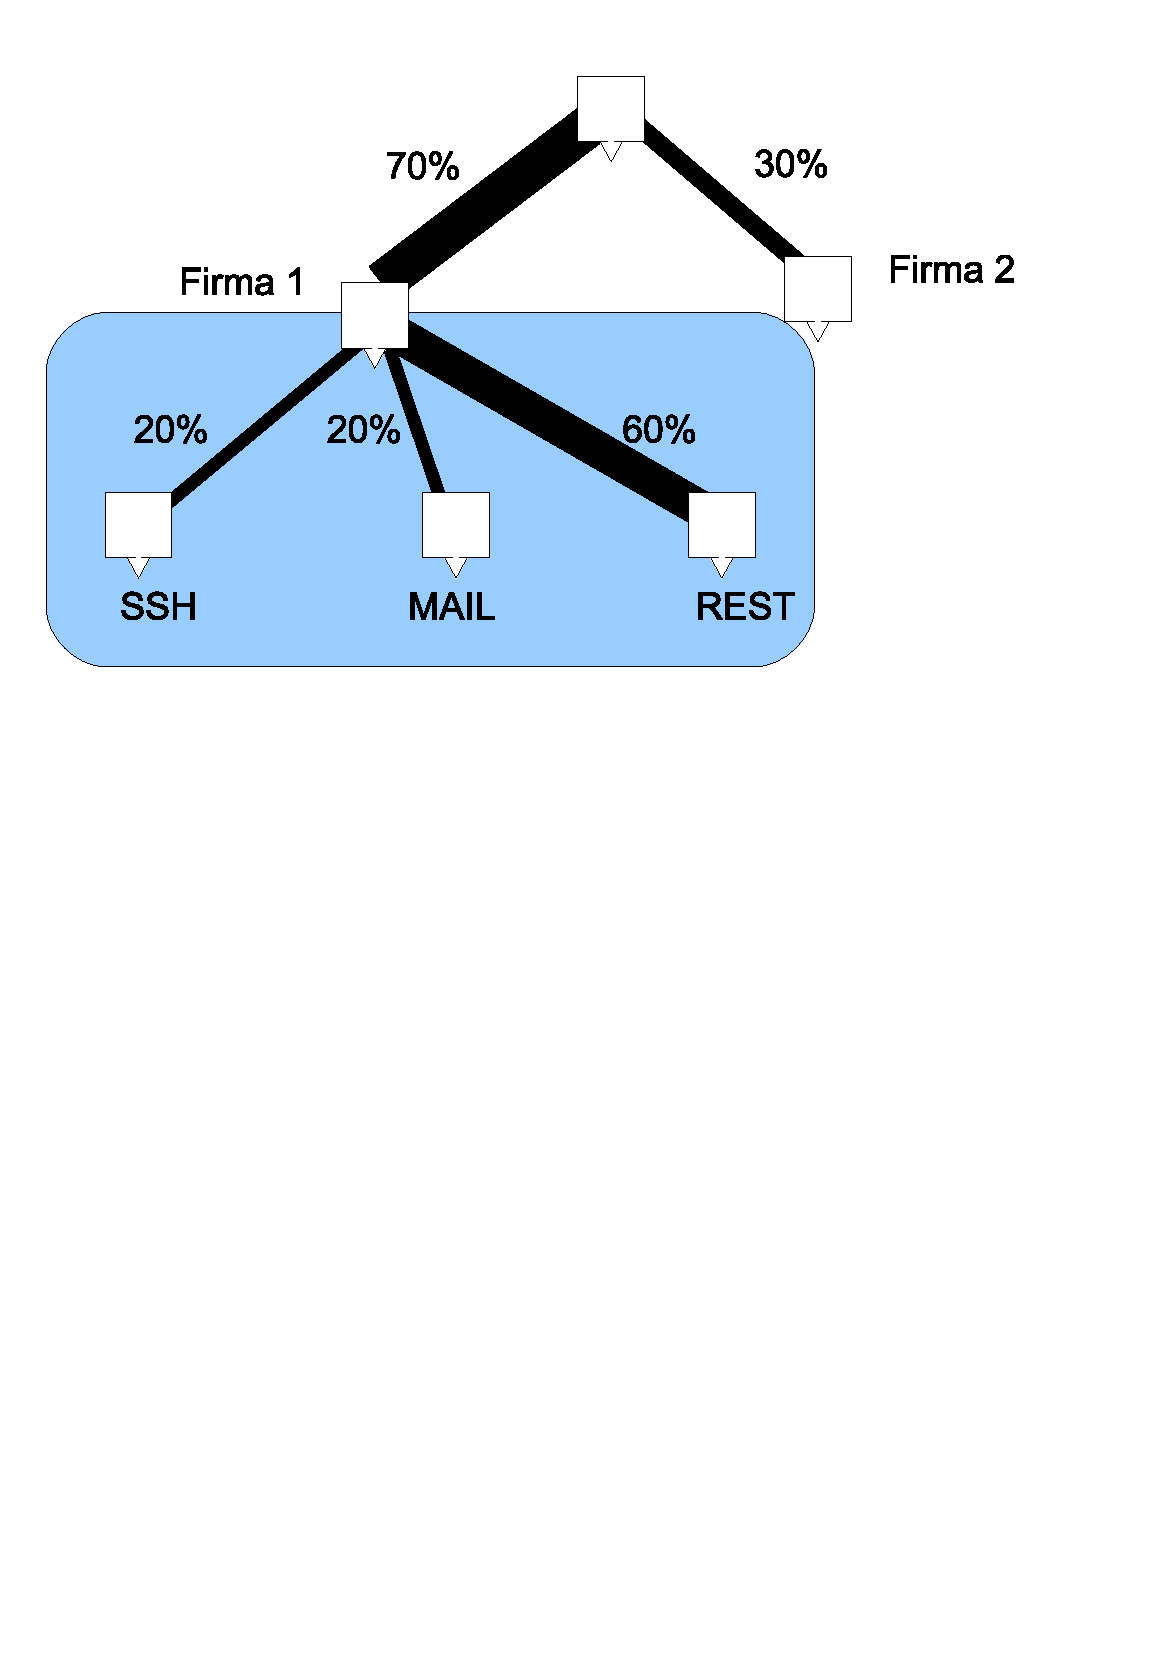
\includegraphics[width=1\textwidth]{GFX/bucket-hiracy-menge_combined}
  \end{figure}
\end{frame}


\section{Rückblick}
%\subsection*{}
\begin{frame}
\frametitle{Rückblick}
\begin{itemize}
  \item Keine automatische Umstellung der Leitung
  %	Parameter, Gegenstelle, Services, Zeit
  \item Verschiebung der Zeitplanung
\begin{itemize}
 \item lange Informationssuche
 \item Wegfall der automatischen Routing-Änderung
\end{itemize}
  \item volle Nutzung der Pufferzeit
  \item Management via SSH ist auch bei starker Auslastung möglich
\end{itemize}
\end{frame}


\section{Aussicht/Erweiterbarkeit}
%\subsection*{}
\begin{frame}
\frametitle{Erweiterung}
\begin{itemize}
  \item Priorisierung der Token Buckets \\$\rightarrow$ stärkere Auslastung der Leitung insgesamt
  % zwei gleich große/starke TB
  \item Management über Webinterface \\$\rightarrow$ direktes Management durch Kunden möglich
\end{itemize}
\end{frame}

\section[]{}


\section[]{}
\begin{frame}
\begin{center}
\Large Vielen Dank für Ihre Aufmerksamkeit!\\Haben Sie noch Fragen?\end{center}
\end{frame}


% You can create overlays
%\begin{itemize}
%  \item using the \texttt{pause} command:
%  \begin{itemize}
%    \item First item.
%    \pause
%    \item Second item.
%  \end{itemize}
%  \item using overlay specifications:
% \begin{itemize}
%    \item<3-> First item.
%    \item<4-> Second item.
%  \end{itemize}
%  \item using the general \texttt{uncover} command:
%  \begin{itemize}
%    \uncover<5->{\item First item.}
%    \uncover<6->{\item Second item.}
%  \end{itemize}
%\end{itemize}


% The following outlook is optional.
%\vskip0pt plus.5fill
%\begin{itemize}
%  \item Outlook
%  \begin{itemize}
%    \item Something you haven't solved.
%    \item Something else you haven't solved.
%  \end{itemize}
%\end{itemize}


\end{document}
